%%%%%%%%%%%%%%%%%%%%%%%%%%%%%%%%%%%%%%%%%%%%%%%%%%%%%%%%%%%%%%%%%
% Master's Thesis in Electrical Engineering
% Music Information Retrieval over Traditional Flute compositions
%%%%%%%%%%%%%%%%%%%%%%%%%%%%%%%%%%%%%%%%%%%%%%%%%%%%%%%%%%%%%%%%%

%----------------------------------------------------------------------------------------
%	PACKAGES AND DOCUMENT CONFIGURATIONS
%----------------------------------------------------------------------------------------

\documentclass{article}

\usepackage[version=3]{mhchem} % Package for chemical equation typesetting
\usepackage{siunitx} % Provides the \SI{}{} and \si{} command for typesetting SI units

\usepackage[english]{babel}
\selectlanguage{english}
\usepackage[utf8]{inputenc}
\usepackage{graphicx} % Required for the inclusion of images
\usepackage{natbib} % Required to change bibliography style to APA
\usepackage{amsmath} % Required for some math elements 

\usepackage{float}

\usepackage{geometry}
 \geometry{
 a4paper,
 total={170mm,257mm},
 left=20mm,
 top=20mm,
 }

\usepackage{listings}
\usepackage{color} %red, green, blue, yellow, cyan, magenta, black, white
\definecolor{mygreen}{RGB}{28,172,0} % color values Red, Green, Blue
\definecolor{mylilas}{RGB}{170,55,241}


\setlength\parindent{0pt} % Removes all indentation from paragraphs

\renewcommand{\labelenumi}{\alph{enumi}.} % Make numbering in the enumerate environment by letter rather than number (e.g. section 6)


%----------------------------------------------------------------------------------------
%	DOCUMENT INFORMATION
%----------------------------------------------------------------------------------------

\title{\textbf{On Music Information Retrieval over Traditional Flute compositions}\\\large \textsc{Master's Thesis in Electrical Engineering} - \textit{Instituto de Ingeniería Eléctrica, Facultad de Ingeniería, Universidad de la República, Uruguay}}

\author{\textit{Juan Braga}}
\date{\today}

\begin{document}

\maketitle 
\begin{abstract}
This present work reports about the extraction of meaningful music events from Traditional Flute \textit{repertoire}. A set of Flute Solo Compositions is selected and labeled for algorithm evaluation. Results are reported using commom mir metrics implemented on \cite{raffel2014mir_eval}.
\end{abstract}


\section{Introduction}

\subsection{Flute Acoustics}

\subsection{Set of selected Solo Flute Compositions}

\subsection{Outline}

\begin{itemize} 
  \item \textit{Blow Hole Covered}: El flujo de aire ingresa directo al tubo de la flauta, sin generar turbulencia contra el filo de la embocadura. 
  \item \textit{Breathy Embrochure}: Caso intermedio entre las otras dos embocaduras. 
  \item \textit{Normal Embrochure}: Embocadura clásica de la flauta, donde el el flujo de aire frente al filo de la embocadura genera la exitación tonal.
\end{itemize}
\medskip

\begin{figure}[H]
\begin{center}
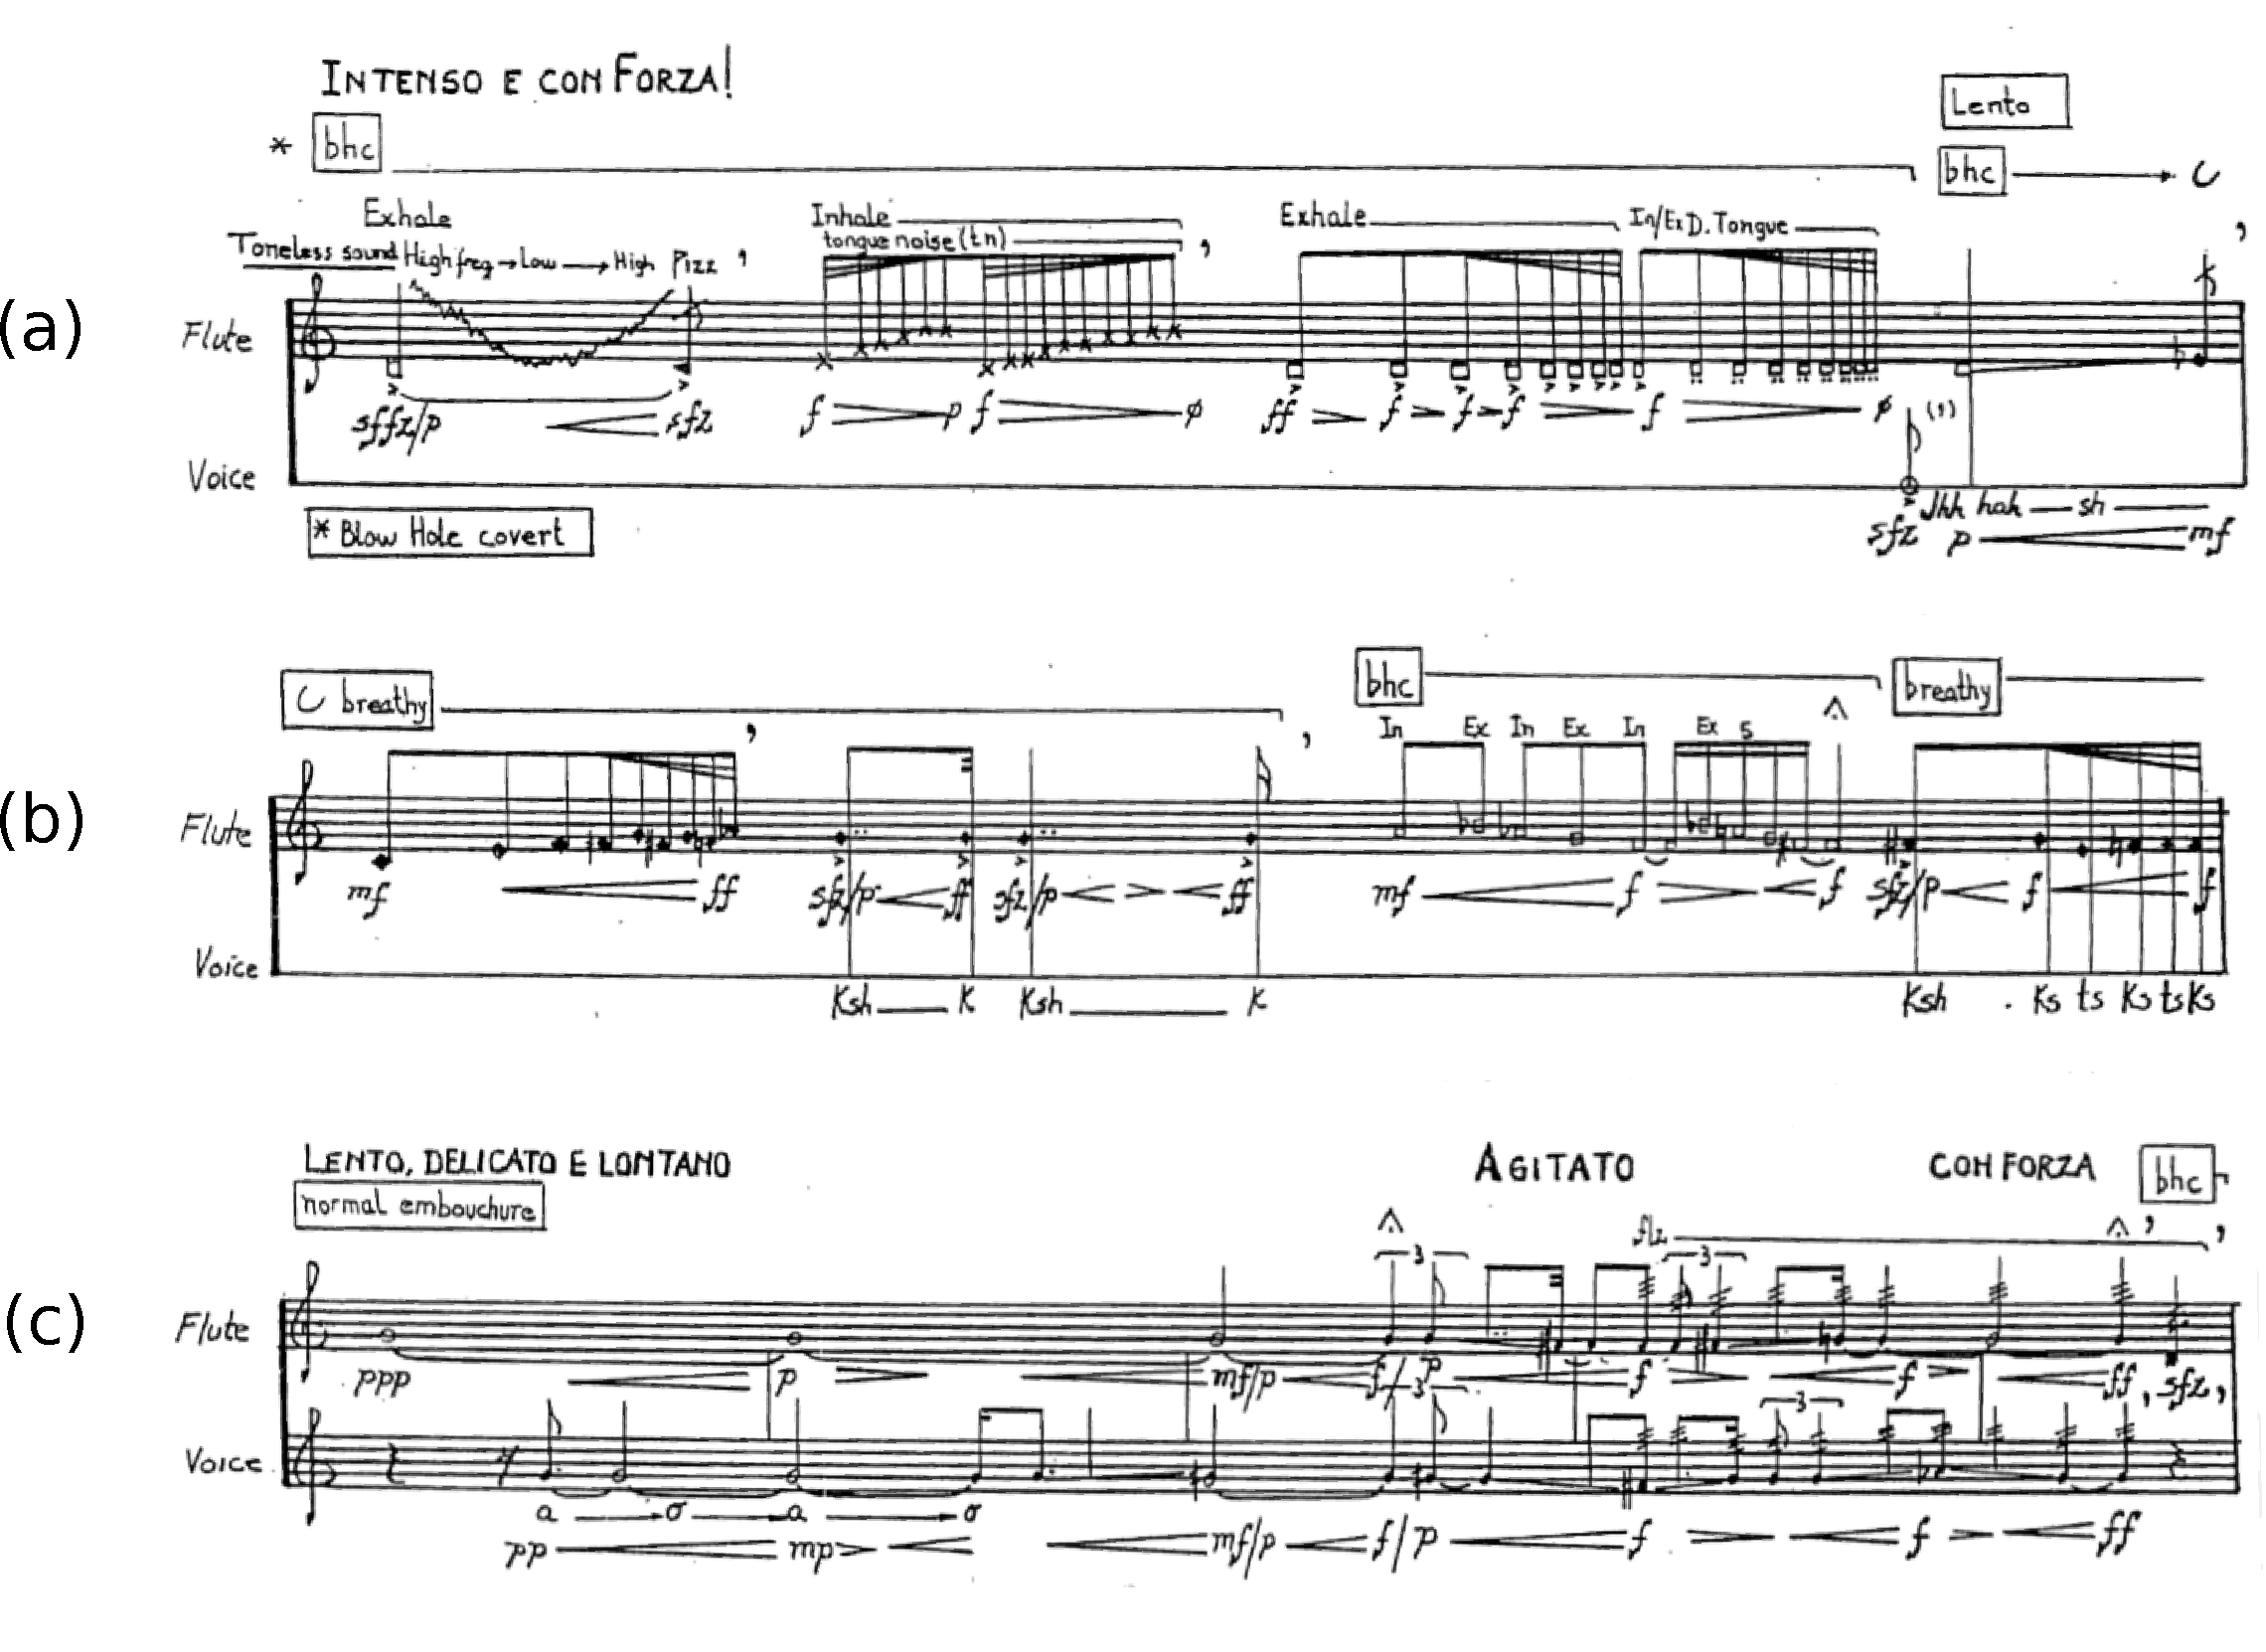
\includegraphics[width=0.9\textwidth]{embocaduras} 
\caption{Notación de las embocaduras se observa en la parte superior de los sistemas. (a) \textit{Blow Hole Covered}. (b) \textit{Breathy Embrochure}. (c) \textit{Normal Embrochure}. Fragmentos extraídos de la partitura de Aliento/Arrugas.}
\label{fig:embocaduras}
\end{center}
\end{figure}

\section*{Definición del Problema}
Se propone la extracción automática del tipo de embocadura a través del análisis computacional de grabaciones de la obra. En este caso se utilizará una estrategia de resolución del tipo de reconocimiento de patrones, en particular de clasificación supervisada. 

\section*{Datos}
Se cuenta con 3 grabaciones de diferentes intérpretes de la obra Aliento/Arrugas. Los intérpretes son: Pablo Somma, Emma Resmini y Ulla Suokko. Los archivos de audio se etiquetaron utilizando el software \textit{Sonic Visualizer} dividiendo los fragmentos de audio en 5 clases:

\begin{itemize} 
  \item Silencio.
  \item Silencio con respiración del intérprete. 
  \item Sonido generado con \textit{Blow Hole Covered}.
  \item Sonido generado con \textit{Breathy Embrochure}.
  \item Sonido generado con \textit{Normal Embrochure}.
\end{itemize}


 


%----------------------------------------------------------------------------------------
%	BIBLIOGRAPHY
%----------------------------------------------------------------------------------------


\newpage
\bibliographystyle{apalike}
\bibliography{biblio}


%----------------------------------------------------------------------------------------
\end{document}


